%!TEX program = xelatex
\documentclass[10pt]{beamer}
\usepackage{tikz}
\tikzset{global scale/.style={
    scale=#1,
    every node/.style={scale=#1}
  }
}
\setcounter{tocdepth}{1}
\usepackage{pgfplots}
\pgfmathdeclarefunction{gauss}{2}{%
  \pgfmathparse{1/(#2*sqrt(2*pi))*exp(-((x-#1)^2)/(2*#2^2))}%
}
\pgfplotsset{compat=1.10}

\def\x{-0.5}
\def\fx{1/(1.3*sqrt(2*pi))*exp(-((\x+0.5)^2)/(2*1.3^2))}
\def\y{1}
\def\fy{1/(0.9*sqrt(2*pi))*exp(-((\y-1)^2)/(2*0.9^2))}


\usetheme[menuwidth={0.7\paperwidth}]{erlangen}
\setbeamercovered{transparent=20}
\setbeamerfont{frametitle}{series=\bfseries}
\usepackage{hyperref}
\hypersetup{colorlinks=false,
            colorlinks=black,
            pdfborder=100,
            citecolor=black}


\setbeamerfont{block title}{series=\bfseries}
\usepackage{graphicx}


\usepackage[no-math,cm-default]{fontspec}
\setmainfont{Minion Pro}
\setsansfont[BoldFont={Myriad Pro Semibold}]{Myriad Pro}
\setmonofont{Courier New}
\usepackage{xeCJK}
\setCJKmainfont[BoldFont={方正黑体简体},ItalicFont={楷体}]{宋体}
\setCJKsansfont[BoldFont={方正黑体简体}]{方正中等线简体}
\setCJKmonofont{方正中等线简体}
\XeTeXlinebreaklocale "zh"
\XeTeXlinebreakskip = 0pt plus 1pt

\usefonttheme[onlymath]{serif}
\usepackage[noamssymbols]{mtpro2}

% \renewcommand\contentsname{目录}
\setbeamertemplate{itemize items}{\raisebox{0.15ex}{\small$\bullet$}}

\begin{document}
\title{Self-Selection and the Earnings of Immigrants}
\subtitle{George J. Borjas (AER, 1987)}
\author[Borjas (AER,1987)]{\small Pre: DENG Dongsheng}
\date{\today}
% \institute{The School of Economics\\
  % \vspace{-0.2em}{\small Fudan University} }

\begin{frame}[plain]
  \titlepage
\end{frame}


\begin{frame}{Table of Contents}
  \tableofcontents
\end{frame}


\section{Introduction}

\begin{frame}{Literature Review}
\textbf{Most convincing finding}: Immigrants do not make up a random sample of the population from the countries of origin;

\begin{enumerate}
    \item  Cross-section earnings functions are estimated with two conclusions:
    \begin{itemize}
        \item the age-earnings profile of immigrants is \alert{steeper} than the that of the native population with the same measured skills;
        \item it \alert{crosses} that of natives about \textit{10-15} years after immigration.
    \end{itemize}
    \item Single cross-section study $\Rightarrow$ studies of cohort or longitudinal data.
    \begin{itemize}
        \item The earnings and years since migration are positively correlated can be explained  \textit{aging effect} (i.e., assimilation) or \textit{cohort differences in quality}.
        \item Single cross-section data cannot separately indentify aging and cohort effects.
    \end{itemize}
\end{enumerate}

\end{frame}

\begin{frame}[c]\frametitle{Motivation}
\textbf{Question}: \textit{how cohort quality and immigrant self-selection are related?}
\begin{itemize}
    \item Immigrants selected from the upper or lower tail?
    \item Does that ensure that they end up in the upper tail of the U.S. income distribution?
    \item What factors are responsible for cohort quality decline?
\end{itemize}

\textbf{Methods and Findings:}
\begin{itemize}
    \item Assumption: income maximizing behavior of the potential migrants.
    \item Upper tail of income conditions are not generally satisfied.
    \item Key variables can predict the types of migrants.
    \item Data: 41 countries using 1970 and 1980 censuses.
    \item A few key economic and political conditions can explain the quality of immigrants.
\end{itemize}

\end{frame}

\section{Theoretical Framwork}
\subsection{Model Setup}
\begin{frame}[c]\frametitle{Basic Setup}
\begin{itemize}
    \item Two countries 0 and 1, denoting the source and host country (U.S.).
    \item Earnings decomposition: observable ($\mu_{i}$) $+$ unobserved ($\varepsilon_{i}$).
    \item Residents of the home country have earnings
    \begin{equation}
        \ln w_{0} = \mu_{0} + \varepsilon_{0}, \quad \varepsilon_{0} \sim N(0,\sigma^{2}_{0})
    \end{equation}
    \item If they were to migrate to U.S., their earnings will be
    \begin{equation}
        \ln w_{1} = \mu_{1} + \varepsilon_{1}, \quad \varepsilon_{1} \sim N(0,\sigma^{2}_{1})
    \end{equation}
\item Correlation btw the source and host country is
\begin{equation*}
    \rho = \frac{\sigma_{01}}{\sigma_{0}\sigma_{1}},\quad \text{where } \sigma_{01} = \mathrm{cov}(\varepsilon_{0},\varepsilon_{1}).
\end{equation*}
\item Cost of migration is $C$, the "time equivalent" terms $\pi = C/w_{0}$, assume it\rq{}s constant.
\end{itemize}
\end{frame}

\subsection{Migration Decision}
\begin{frame}[c]\frametitle{Migration Decision}

\begin{itemize}
    \item Index function:
    \begin{equation}
        I = \ln\big(w_{1}/(w_{0}+C)\big)\approx (\mu_{1}-\mu_{0} - \pi) + (\varepsilon_{1} - \varepsilon_{0})
    \end{equation}
    \item \alert{\textbf {Self-Selection Decision Rule:}}
    \begin{equation*}
        (\mu_{1} - \mu_{0} -\pi) + (\varepsilon_{1} - \varepsilon_{0}) > 0
    \end{equation*}
    \item Emigration rate is given by
    \begin{equation}
        P = \mathrm{Pr}\big[v > -(\mu_{1} - \mu_{0} - \pi)\big] = 1- \Phi(z)
    \end{equation}
    where $v=\varepsilon_{1}-\varepsilon_{0}; z=(\mu_{0}-\mu_{1}+\pi)/\sigma_{v}$
    \item the higher is $z$, the lower is the prob of migration.
    \begin{equation*}
        \frac{\partial P}{\partial \mu_{0}} < 0, \; \frac{\partial P}{\partial \mu_{1}} > 0, \; \frac{\partial P}{\partial \pi} <0.
    \end{equation*}

\end{itemize}

\end{frame}

\subsection{Selction Conditions}
\begin{frame}[c]\frametitle{Average Earnings}
\begin{itemize}
\item Average earnings of emigrants in country 0 v.s. in U.S. are given by
\begin{align}
    E[\ln w_{0} \mid \text{Immigrate}] &= \mu_{0} + \frac{\sigma_{0}\sigma_{1}}{\sigma_{v}}\big(\rho - \frac{\sigma_{0}}{\sigma_{1}}\big) \lambda \label{eq:5}\\
    E[\ln w_{1} \mid \text{Immigrate}] &= \mu_{1} + \frac{\sigma_{0}\sigma_{1}}{\sigma_{v}}\big(\frac{\sigma_{1}}{\sigma_{0}} - \rho \big) \lambda  \label{eq:6}
\end{align}
where $\lambda = \phi(z)/(1-\Phi(z))$, denote $k = \sigma_{1}/\sigma_{0}$.
\item Let $Q_{0}$ be income differential btw average emigrant and average person in country 0, $Q_{1}$ income differential btw that and the average native person in U.S..
\item by \eqref{eq:5} and \eqref{eq:6},
\begin{align*}
    Q_{0} &=  \frac{\sigma_{0}\sigma_{1}}{\sigma_{v}}\big(\rho - \frac{\sigma_{0}}{\sigma_{1}}\big) \lambda = \frac{\sigma_{0}\sigma_{1}}{\sigma_{v}}\big(\rho - \frac{1}{k}\big) \lambda \\
    Q_{1} &=   \frac{\sigma_{0}\sigma_{1}}{\sigma_{v}}\big(\frac{\sigma_{1}}{\sigma_{0}} - \rho \big) \lambda =  \frac{\sigma_{0}\sigma_{1}}{\sigma_{v}}\big(k - \rho \big) \lambda
\end{align*}

\end{itemize}
\end{frame}

\begin{frame}[c]\frametitle{Selction Conditions}
\begin{center}
\begin{tikzpicture}[global scale=0.8]
\draw[->] (-4.2,0) -- (4.2,0) node[below]{$Q_{0}$};
\draw[->] (0,-4.2) -- (0,4.2) node[right]{$Q_{1}$};
\draw (0,0) node[anchor=north west]{$(0,0)$};
\visible<1->{
\fill[gray,opacity=0.2] (0,0) rectangle (4,4);
\draw (2,2) node[text width=3cm,align=center]{\alert{Postive Selection} $\rho > 1/k \mbox{ and } k > 1$};}
\visible<2->{
\fill[gray,opacity=0.2] (0,0) rectangle (-4,-4);
\draw (-2,-2) node[text width=3cm,align=center]{\alert{Negative Selection} $\rho > k \mbox{ and } k < 1$};}
\visible<3->{
\fill[gray,opacity=0.2] (0,0) rectangle (-4,4);
\draw (-2,2) node[text width=3cm,align=center]{\alert{Refugee Sorting} $\rho < \min\{1/k,k\}$}; }
\visible<4->{
\fill[gray,opacity=0.2] (0,0) rectangle (4,-4);
\draw (0.2,-0.2) -- (3.8,-3.8);
\draw (3.8,-0.2) -- (0.2,-3.8);
\draw (2,-2) node[text width=5cm,align=center]{\alert{Theoretically Impossible} };}
\visible<5-6>{
\fill[erlangenblue,opacity=0.5] (0,-4) rectangle (4,4);
\draw (2,0) node[text width=3cm,align=center]{\textcolor{white}{Upper tail of home country} };}
\visible<6-6>{
\fill[erlangenblue,opacity=0.5] (0,-4) rectangle (-4,4);
\draw (-2,0) node[text width=3cm,align=center]{\textcolor{white}{Lower tail of home country} };}
\visible<7-8>{
\fill[erlangenlyellow,opacity=0.4] (-4,0) rectangle (4,4);
\draw (0,1) node[text width=3cm,align=center]{\textcolor{erlangenblue}{Outperform the native population} };}
\visible<8-8>{
\fill[erlangenlyellow,opacity=0.4] (-4,0) rectangle (4,-4);
\draw (0,-1) node[text width=3cm,align=center]{\textcolor{erlangenblue}{Not well performed  in U.S. labor market} };}
\end{tikzpicture}
\end{center}
\end{frame}


\begin{frame}[c]\frametitle{Quality of Immigrants}
Reduced-form quality of immigrants equation given by
\begin{equation}
    Q_{1} = Q_{1} (\mu_{1} - \mu_{0} -\pi,\sigma_{0},\sigma_{1},\rho).
\end{equation}
$Q_{1} = \gamma \lambda$, where $\gamma = (\sigma_{0}\sigma_{1}/\sigma_{v})/(k-\rho)$, $\lambda = \phi(z)/(1-\Phi(z))$.
\begin{itemize}
    \item $\gamma$ not depend on the size of flow;
    \item $\lambda$ does.
\end{itemize}

\textbf{Effect Decomposition:}
\begin{equation}
    \frac{\partial Q_{1}}{\partial \alpha} = \lambda \frac{\partial \gamma}{\partial \alpha} + \gamma \frac{\partial \lambda}{\partial \alpha}.
\end{equation}
\begin{itemize}
    \item The first term is called \alert{composition} effect;
    \item The second term is \alert{scale} effect.
\end{itemize}

\end{frame}
\subsection{Comparative statics}
\begin{frame}[c]\frametitle{$\alpha$: Home Country's Income}
What happens to immigrant quality as the mean of the home country's income distribution increases?
\begin{equation}
    \frac{\partial Q_{1}}{\partial \mu_{0}} = \frac{\sigma_{1}\sigma_{0}}{\sigma_{v}^{2}}(k-\rho)\frac{\partial \lambda}{\partial z}.
\end{equation}
\begin{itemize}
    \item Shifts in  $\mu_{0}$ lead only to a scale effect on  $Q_{1}$;
    \item If $k - \rho <0$, then it\rq{}s negative selection ($Q_{1} < 0, k < 1, \rho > k$);
    \item $\partial Q_{1} /\partial \mu_{0} <0$, reason: $\mu_{0}$ increases, the emigration rate falls, since negative selection $\Rightarrow$ reduction of average quality.
\end{itemize}

\end{frame}

\begin{frame}[c]\frametitle{$\alpha$: Home Country's Income Inequality}
Effect of a mean-preserving increase in the income inequality of the home country is given by:
\begin{equation}
    \frac{\partial Q_{1}}{\partial \sigma_{0}} = \frac{\sigma_{1}^{2}\sigma_{0}}{\sigma_{v}^{3}}(\rho^{2}-1)\lambda - \frac{\sigma_{1}\sigma_{0}^{2}}{\sigma_{v}^{3}}(k-\rho)(1-\rho k)\frac{\partial \lambda}{\partial z} z.
\end{equation}

\begin{center}
\begin{tikzpicture}[global scale = 0.85]
\begin{axis}[axis x line=none, axis y line = none,xtick=\empty,ytick=\empty,every axis plot post/.append style={domain=-5:5,samples=50,smooth}] % All plots: from -2:2, 50 samples, smooth, no marks
  % axis x line*=bottom]%, % no box around the plot, only x and y axis
  % enlargelimits=upper] % extend the axes a bit to the right and top
  \addplot[erlangenlyellow] {gauss(1,0.9)};
  \addplot[erlangendarkblue] {gauss(-0.5,1.3)};
  \draw (axis cs:-5,0) -- (axis cs:5,0);
  \draw[dashed] (axis cs:{\x},{\fx}) -- (axis cs:{\x},0) node[below]{$\mu_{0}+\pi$};
  \draw[dashed] (axis cs:{\y},{\fy}) -- (axis cs:{\y},0) node[below]{$\mu_{1}$};
  \node at (axis cs: -3, 0.3){$\sigma_{1} < \sigma_{0}$};
  \only<2->{\addplot[blue] {gauss(-0.5,1.8)};
  \node at (axis cs: -3, 0.2){\textcolor{blue}{$\sigma_{0}^{\prime} > \sigma_{0}$}};}
\end{axis}

\end{tikzpicture}
\end{center}

\end{frame}

\begin{frame}[c]\frametitle{$\alpha$: Home Country's Income Inequality II}

\begin{itemize}
    \item First term is \alert{composition effect}, always be nonpositive ($|\rho|<1$).
    \item $\sigma_{0}$ increases, reduce the income of poorest, and improve the richest.
    \item Change in $\sigma_{0}$ changes the rate of emigration.
    \item Scale effect depends on $(k-\rho)$, $(1-\rho k)$ and $z$.
    \item Under negative selection, $k-\rho <0$ and $1-\rho k >0$.
    \item If $\mu_{1} > \mu_{0} + \pi$, then $z < 0$, \alert{scale effect} is negative.
\end{itemize}

\textbf{Conclusion:} Immigrants from countries with more income inequality will perform worse in the United States.



\end{frame}

\begin{frame}[c]\frametitle{$\alpha$: Correlation Coefficient}

Changes in the correlation coefficient also induce two effects.
\begin{equation}
    \frac{\partial Q_{1}}{\partial \rho} = - \frac{\sigma_{1}\sigma_{0}^{3}}{\sigma_{v}^{3}}(1-\rho k) \lambda + \frac{\sigma_{1}^{2}\sigma_{0}^{2}}{\sigma_{v}^{2}}(k-\rho)\frac{\partial \lambda}{\partial z} z.
\end{equation}
\begin{itemize}
    \item Its sign depends on $-(1-\rho k)$, negative when negative selection.
    \item An increase in $\rho$ implies that a better match exists between performance in the United States and in the home country.
    \item $\sigma_{0} > \sigma_{1}$ decreases the  profitability  of migration for the best persons in country 0 and increases it for the worst persons.
    \item Under negative selection, $k-\rho <0$, $\Rightarrow$ the scale effect depends on the sign of $-z$.
    \item $z < 0$, then scale effect is positive.
\end{itemize}

\end{frame}

\begin{frame}[c]\frametitle{Summary of Comparative Statics}

\centerline{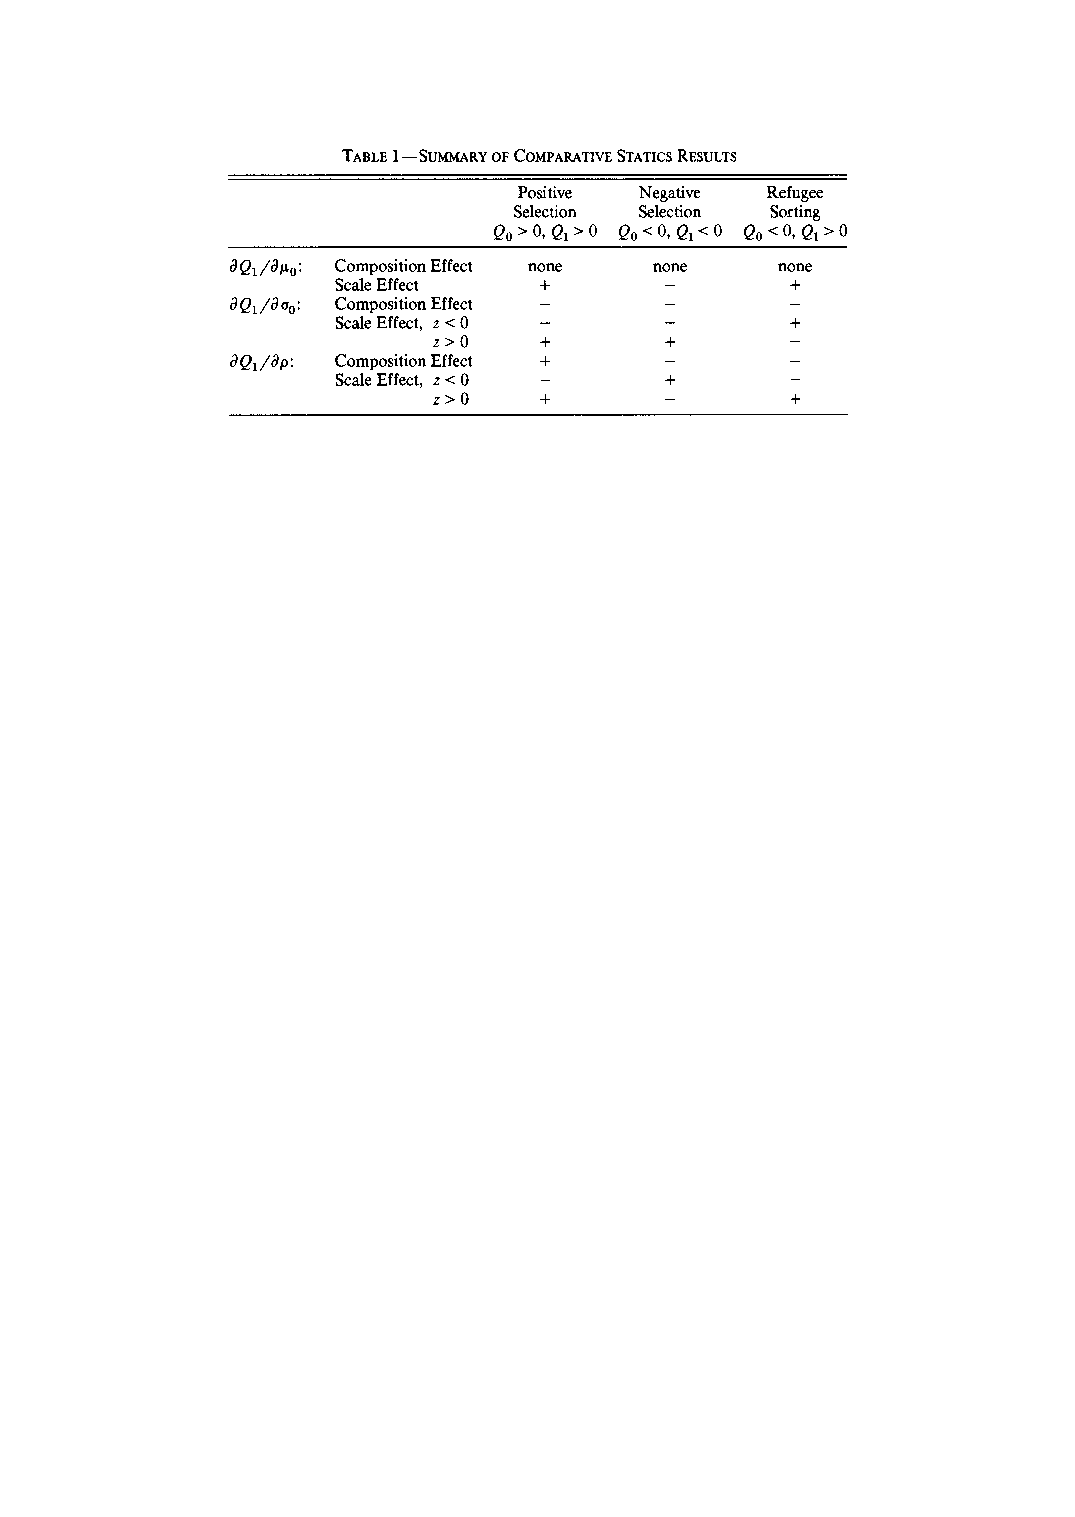
\includegraphics[width=0.9\textwidth]{summary.pdf}}
\begin{enumerate}
    \item Generalizations about the quality of immigrants in the United States are hard to come by.
    \item The model isolate the key factors that determine the types of selections in the immigrant population.
    \item These factors shed light on the finding that the quality of immigrants declined in the postwar period.
\end{enumerate}

\end{frame}

\section{Empirical Framework}
\begin{frame}[c]\frametitle{Specification of Regression Model}
Wage differential is affected by two factors
\begin{enumerate}
    \item differences in the skill composition of the various immigrant cohorts;
    \item the rate of convergence between foreign- and native-born earnings (i.e., the rate of assimilation of immigrants).
\end{enumerate}

An empirical framework regression model specification:
\begin{align}
    \ln w_{i}(T) = X_{i} \theta_{T} &+ \delta I_{i} + \alpha_{1} I_{i} y_{i} + \alpha_{2} I_{i} y_{i}^{2}\notag \\
    &+ \beta_{1} I_{i}C_{i} + \beta_{2}I_{i}C_{i}^{2} + v_{i}. \label{eq:15}
\end{align}
$\alpha_{i}$ captures the impact of assismilation, while $\beta_{i}$ captures the cohort differentials. Since $T\equiv C_{i} + y_{i}$, substituting this identity in \eqref{eq:15} yields
\begin{align}
    \ln w_{i}(T) = X_{i}\theta_{T} &+ (\delta+\beta_{1}T+\beta_{2}T^{2}) I_{i} \notag \\
    &+ (\alpha_{1}-\beta_{2}-2 \beta_{2}T)I_{i}y_{i}\notag\\
    &+ (\alpha_{2}+\beta_{2})I_{i}y_{i}^{2} + v_{i}.
\end{align}

\end{frame}

\begin{frame}[c]\frametitle{Parameters of Interest}
Let $\gamma_{1} = \delta + \beta_{1} T + \beta_{2} T^{2}$, $\gamma_{2} = \alpha_{1} - \beta_{1} -2 \beta_{2}T$, and $\gamma_{3} = \alpha_{2} + \beta_{2}$. This vector will shift over time since
\begin{align}
    \partial \gamma_{1} / \partial T &= \beta_{1} + 2 \beta_{2} T\\
    \partial \gamma_{2} / \partial T &= -2 \beta_{2}\\
    \partial \gamma_{3} / \partial T &= 0
\end{align}

\begin{enumerate}
    \item The earnings function is inherently unstable(structural changes).
    \item Use the 1970 and 1980 census to identify the parameters of interest $(\delta,\alpha_{1},\alpha_{2},\beta_{1},\beta_{2})$.
    \item From these estimates, calculate measures of three alternative dimensions of cohort quality.
\end{enumerate}

\end{frame}

\begin{frame}[c]\frametitle{Dimensions of Cohort Quality}

Three alternative dimensions of cohort quality that underlie the discussion.
\begin{enumerate}
    \item The predicted wage differential in 1979 between the most recently arrived immigrant cohort and the native base.
    \item The rate of wage growth (relative to natives) for an immigrant cohort that has resided in the U.S. for ten years, i.e.  assimilation effect evaluated at $y=10$, given by $\big(\partial \ln w/\partial y\big)|_{y=10}=\alpha_{1} + 20 \alpha_{2}$.
    \item The predicted wage differential immediately after immigration between the 1979 cohort and the 1955 cohort, given by $24(\beta_{1} + 2 \beta_{2}T-24 \beta_{2})$, where $T=1980$。
\end{enumerate}


\end{frame}

\section{Regression Results}
\begin{frame}[c]\frametitle{Data}

\begin{itemize}
    \item Data: 1970 U.S. census and 1980 census;
    \item Restriction: men aged 25-64;
    \begin{itemize}
    \item Employed in the calender year prior the census;
    \item Not Self-Employed or working without pay.
    \item Not in the Armed Forces;
    \item Not reside in group quarters.
    \end{itemize}
    \item 41 countries were selected with $N>80$, account for $90.4\%$ of all immigration to the U.S. btw 1951-1980.
    \item The socioeconomic vector of characteristics $X$ included: years of completed schooling, age, age squared, whether health limits work, whether married, spouse present, and whether resident of an SMSA.
\end{itemize}


\end{frame}

\begin{frame}[t]{Summary of Immigration Flows}

\centerline{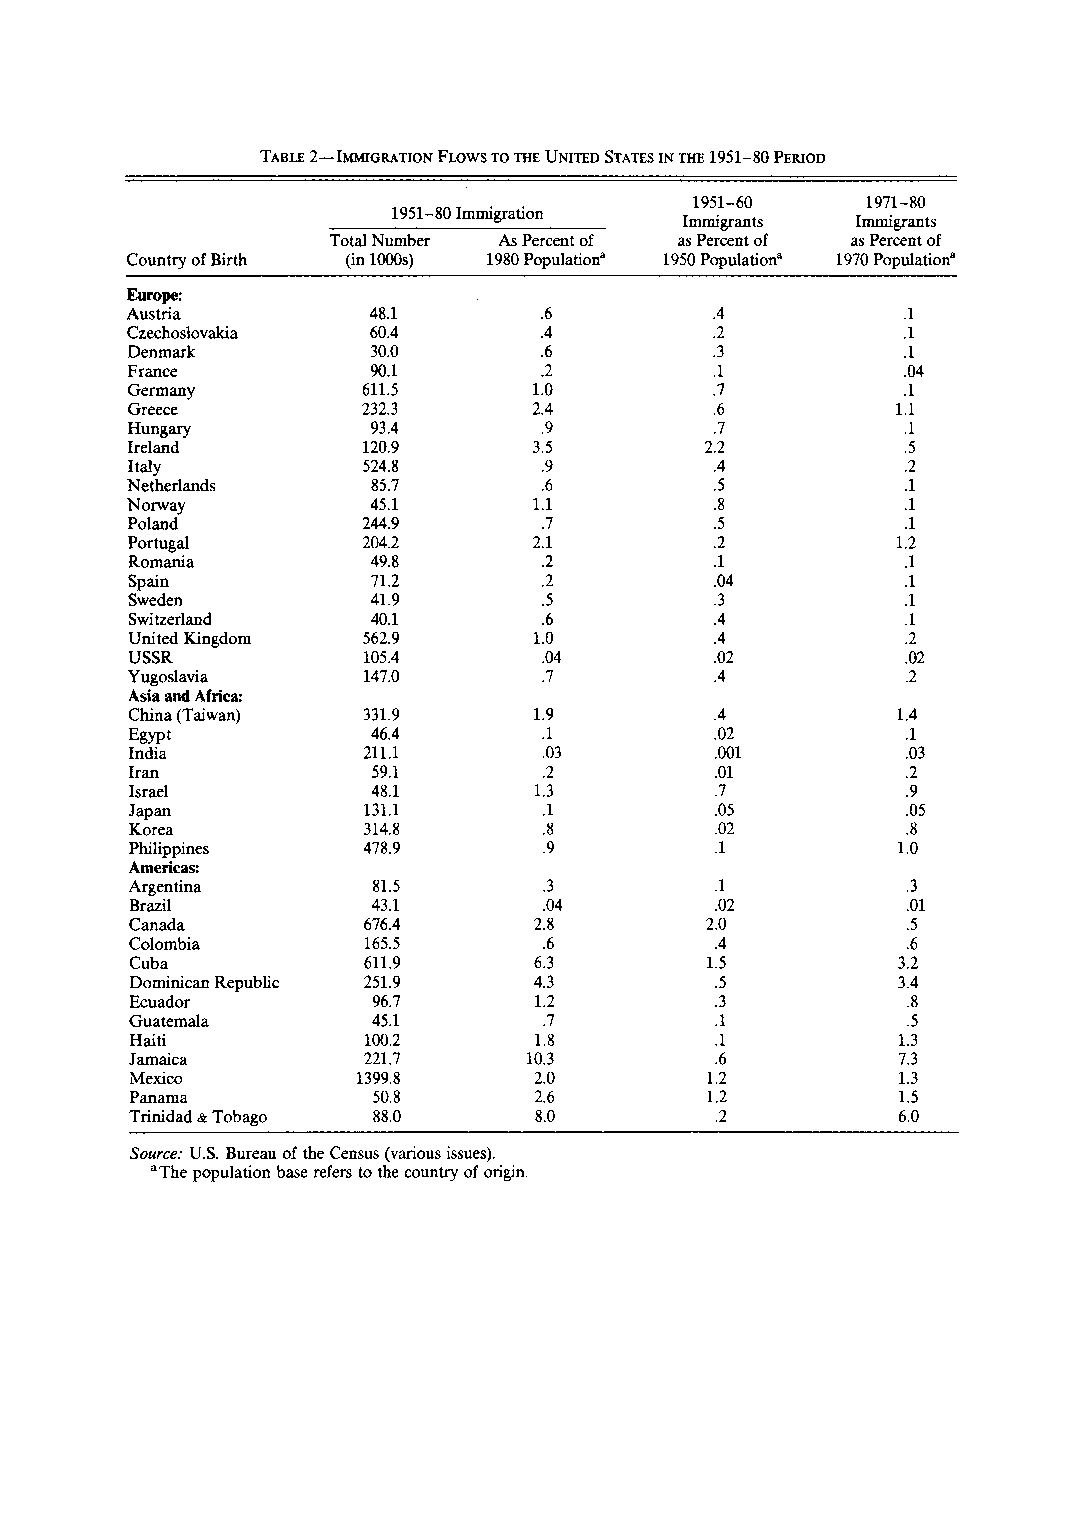
\includegraphics[height=0.9\textheight]{ImmigrationFlow.pdf}}

\end{frame}

\begin{frame}[t]\frametitle{Estimates of Model Parameters}

\centerline{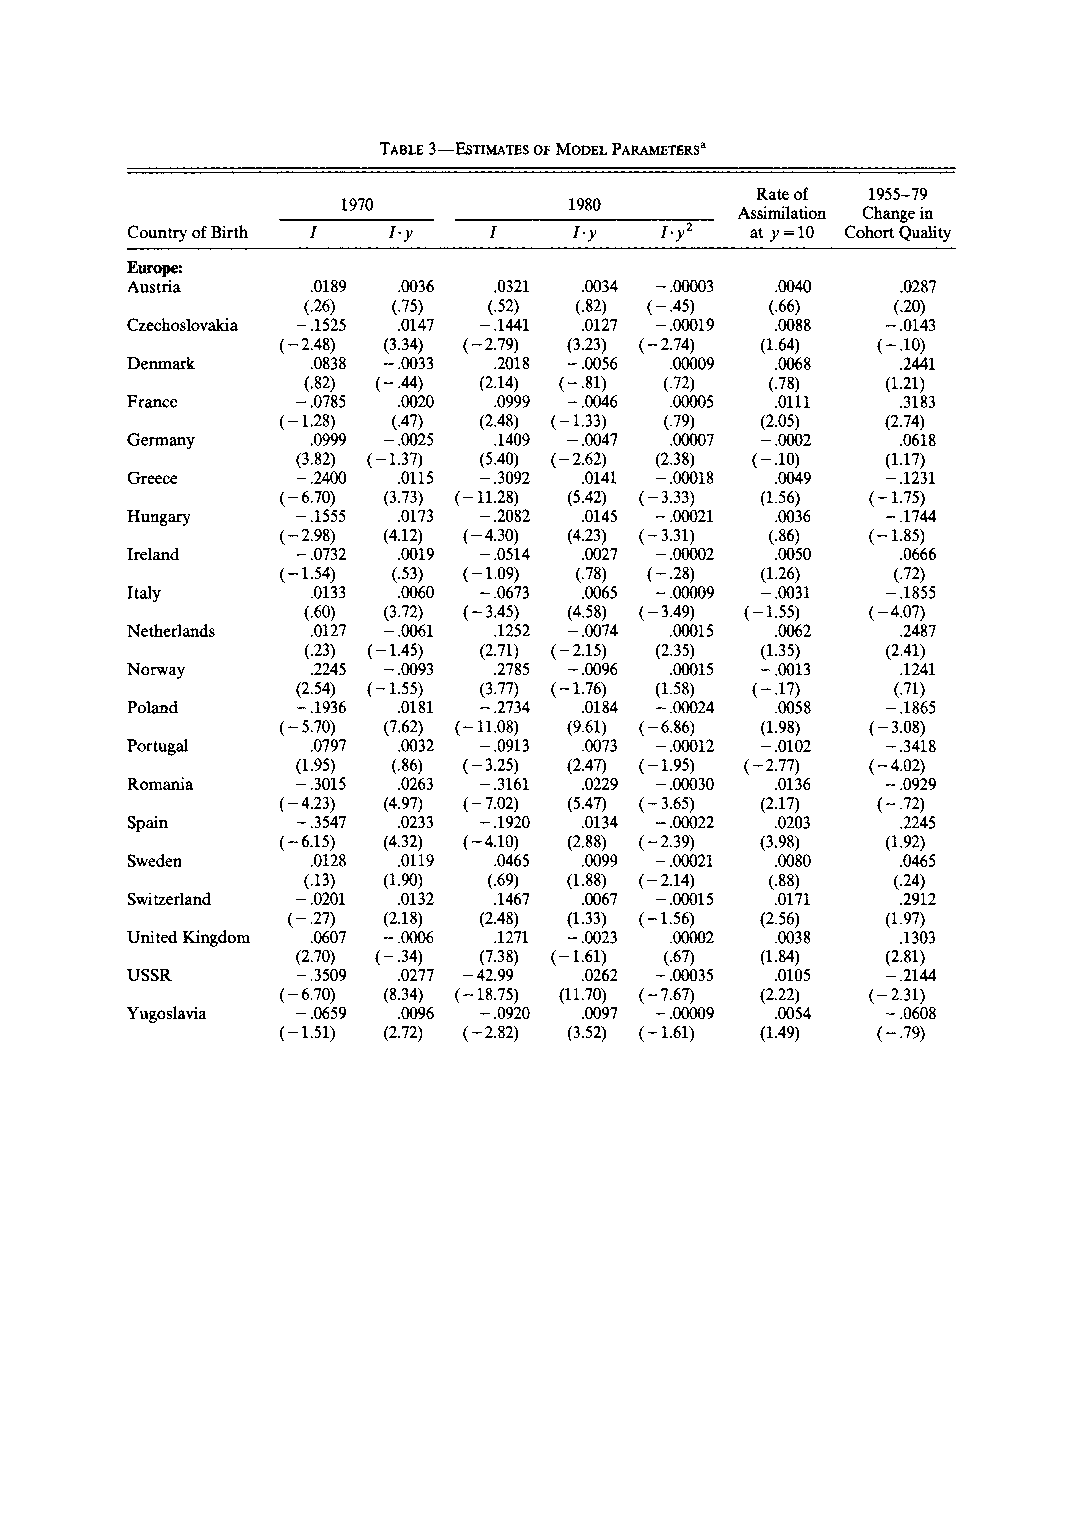
\includegraphics[height=0.9\textheight]{ModReg1.pdf}}

\end{frame}

\begin{frame}[t]\frametitle{Estimates of Model Parameters II}

\centerline{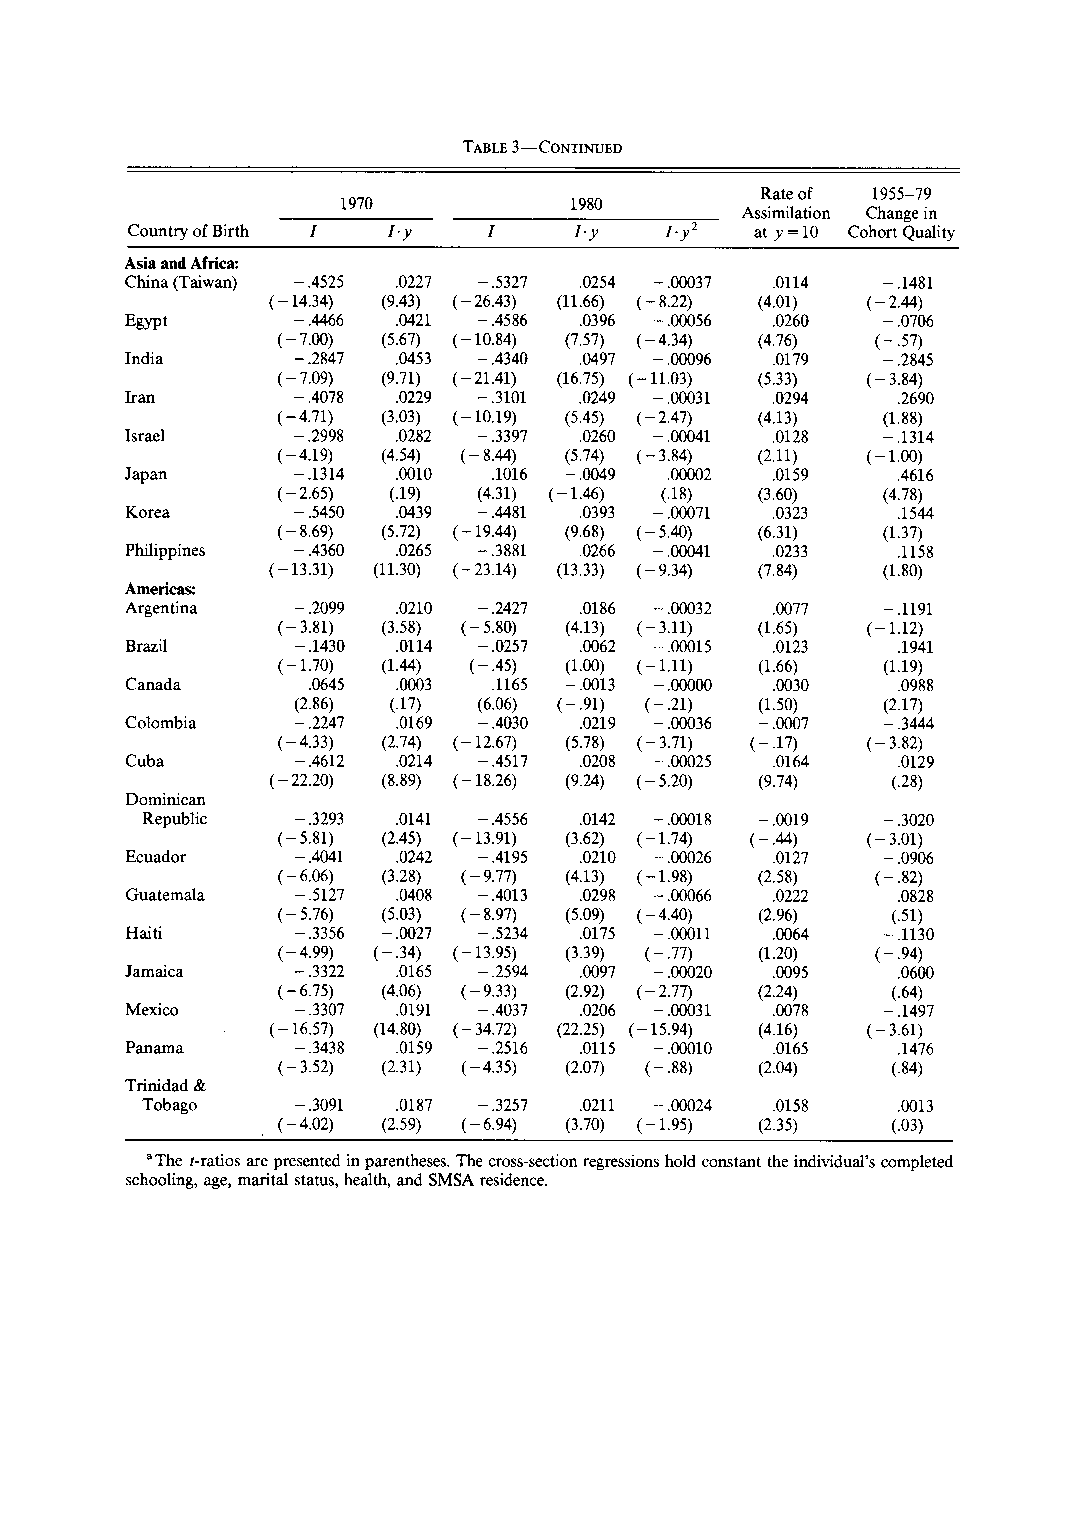
\includegraphics[height=0.9\textheight]{ModReg2.pdf}}

\end{frame}

\section[Determinants]{Determinants of Immigrant Quality}
\begin{frame}[t]{Determinants of Immigrant Quality}
\centerline{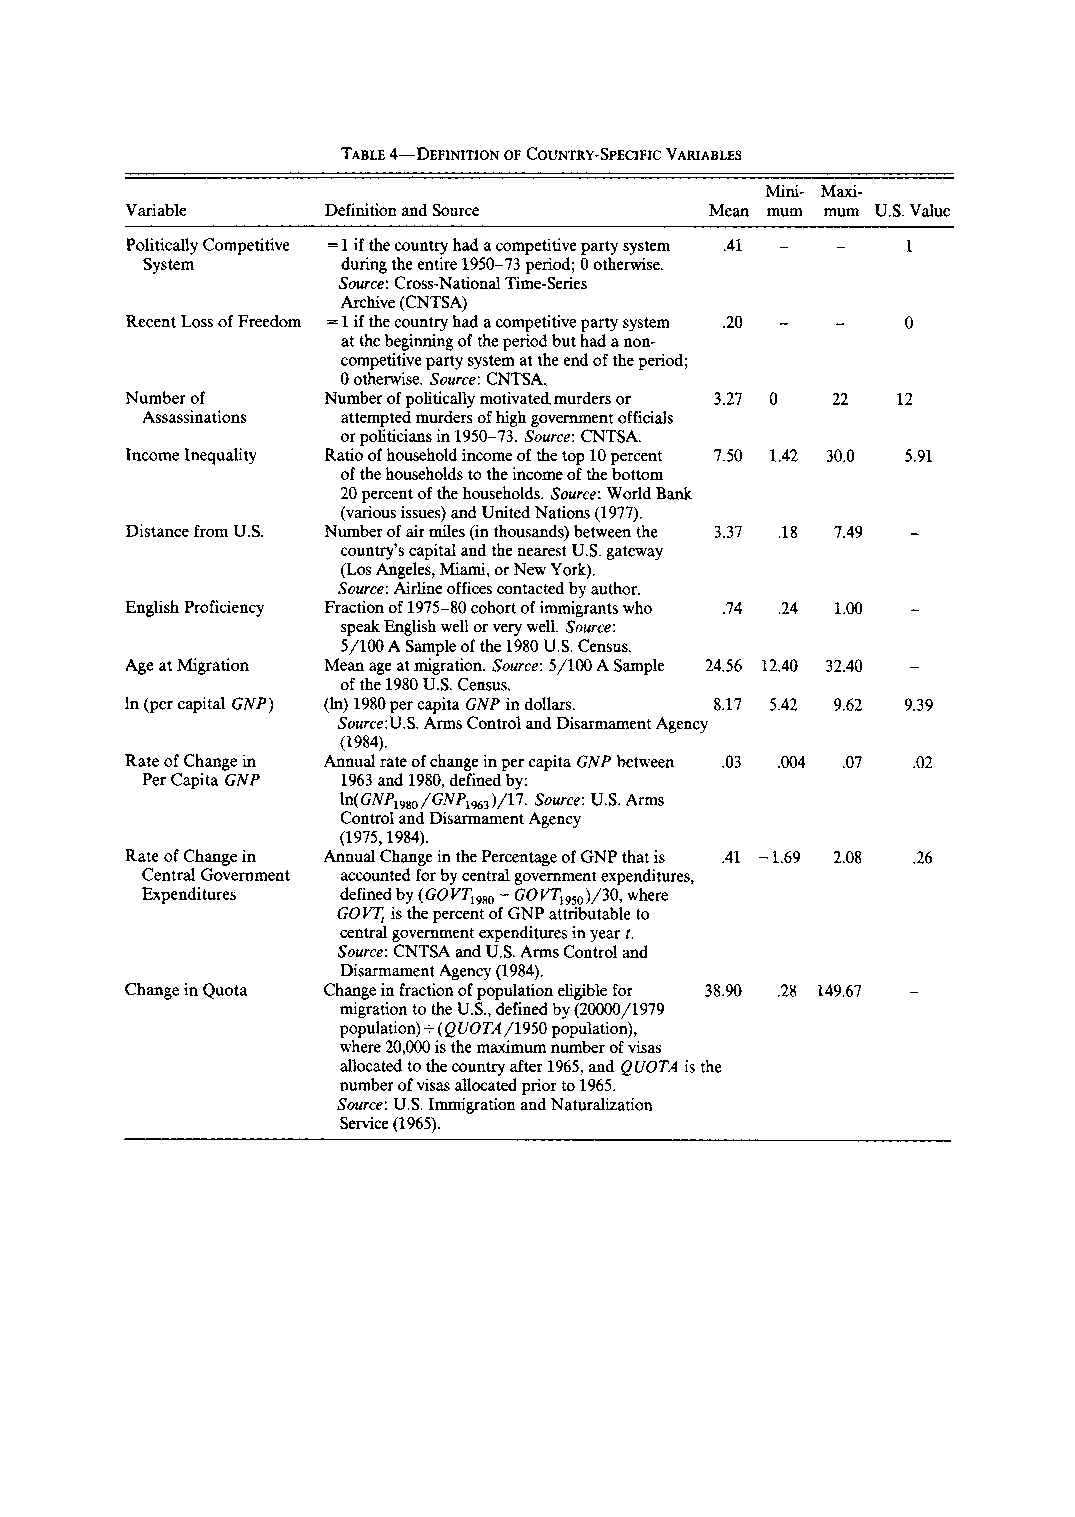
\includegraphics[height=0.85\textheight]{CountrySpe.pdf}}
\end{frame}

\begin{frame}[c]\frametitle{Determinants of the Entry Wage Differential}

\centerline{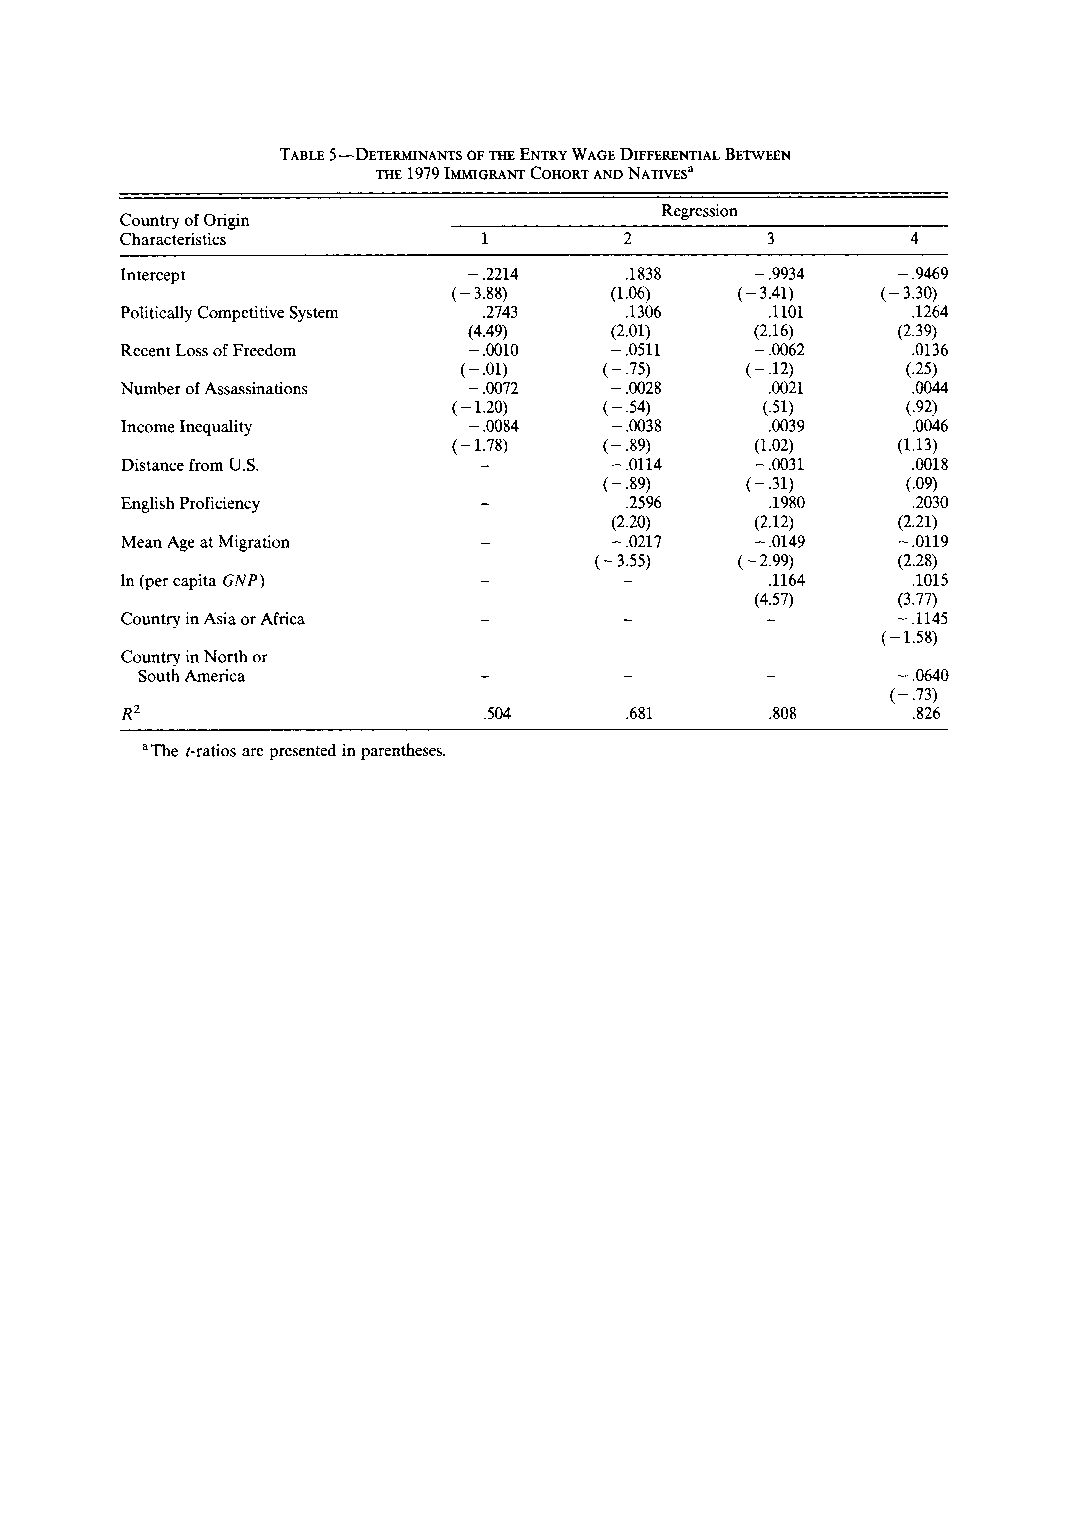
\includegraphics[width=0.85\textwidth]{DetReg1.pdf}}

\end{frame}



\begin{frame}[c]\frametitle{Determinants of the Rate of Assimilation}

\centerline{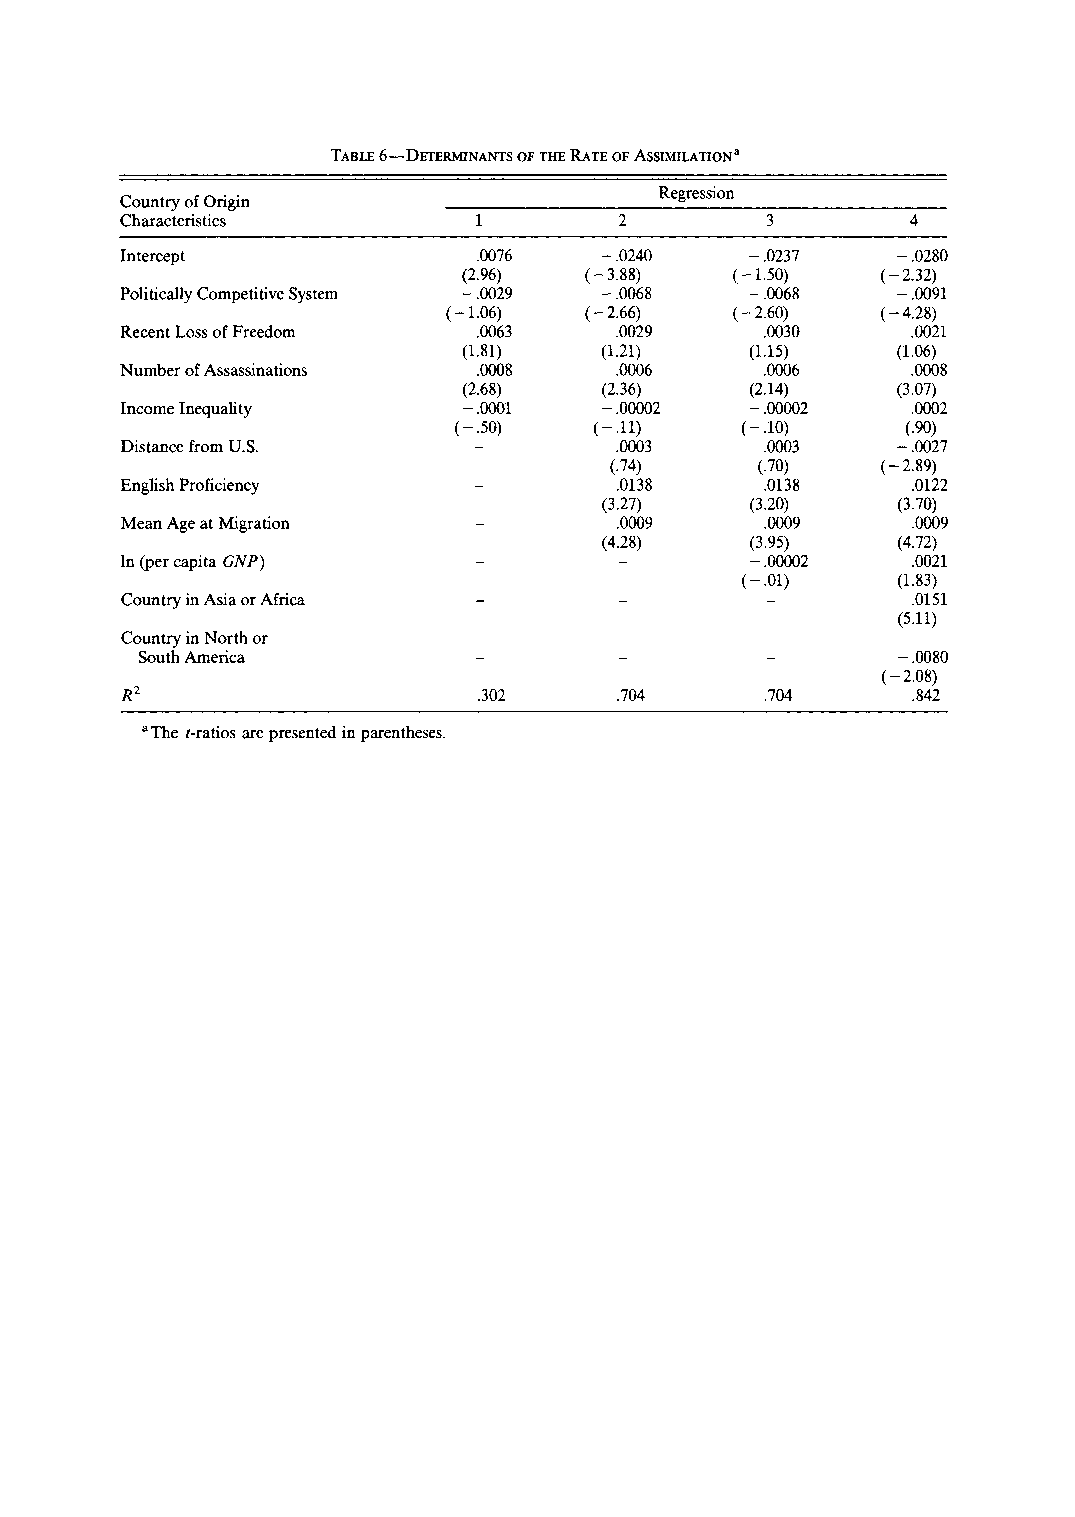
\includegraphics[width=0.85\textwidth]{DetReg2.pdf}}

\end{frame}


\begin{frame}[c]\frametitle{Determinants of the Change in Cohort Quality}

\centerline{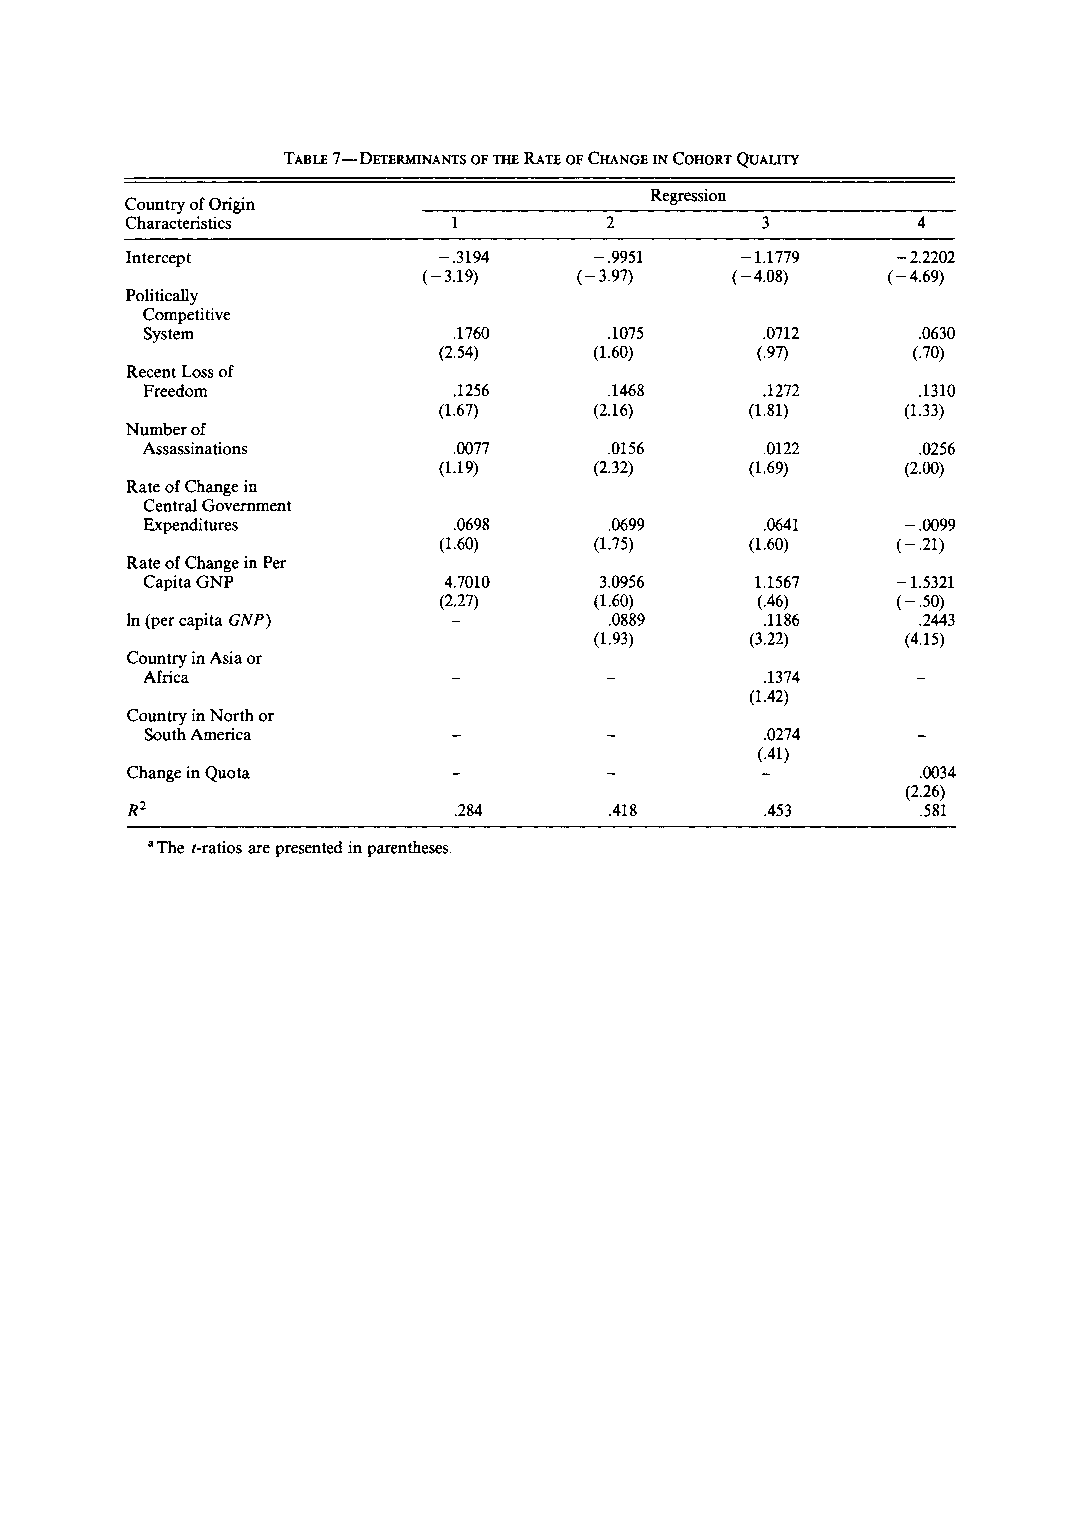
\includegraphics[width=0.8\textwidth]{DetReg3.pdf}}

\end{frame}

\begin{frame}[c]\frametitle{Determinants of the Emigration Rate}

\centerline{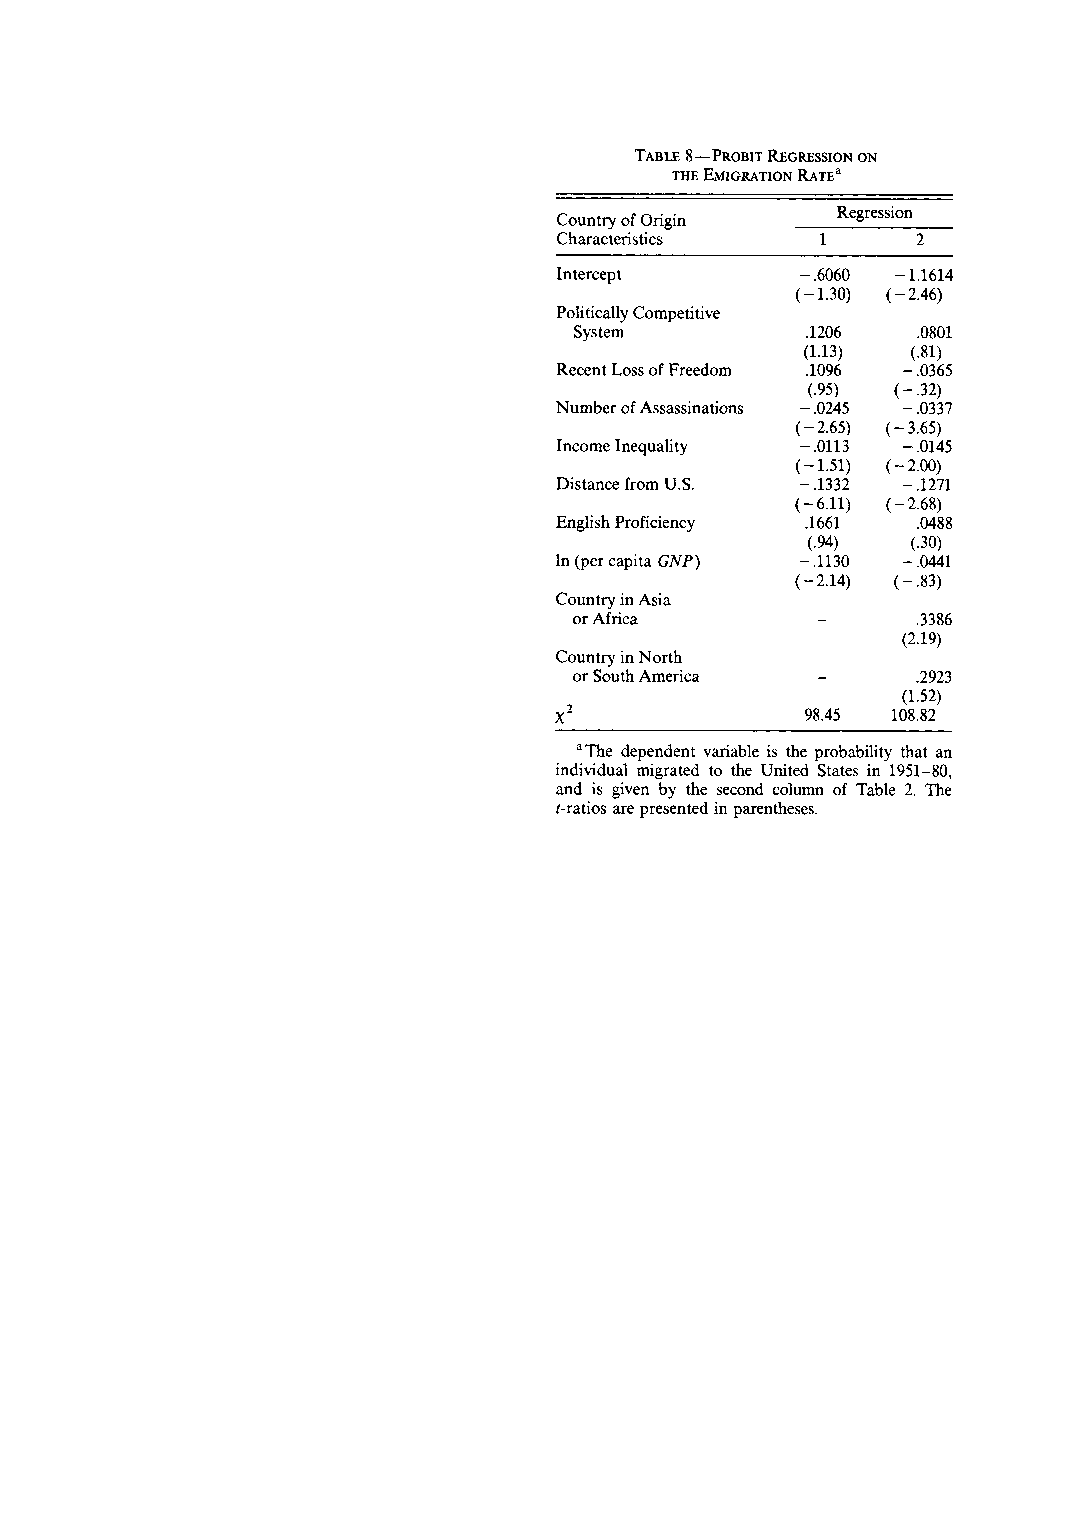
\includegraphics[height=0.8\textheight]{ProbReg.pdf}}

\end{frame}

\section[Summary]{Summary \& Remarks}
\begin{frame}[c]\frametitle{Summary}
\begin{enumerate}
    \item Foreign-born persons in the U.S. need not be drawn from the most able and most ambitious in the country of origin.
    \begin{itemize}
        \item A strong positive correlation between the earnings in home country and the U.S. $(\rho > 1/k)$;
        \item The U.S. has a more unequal income distribution than the home country $(k>1)$.
    \end{itemize}
    \item  Strong country-specific fixed effects in the quality of foreign-born persons;
    \begin{itemize}
        \item Western European countries V.S. less developed countries.
    \end{itemize}
    \item A few variables describing political and economic conditions explain over $2/3$ of the intercountry variance in the mean U.S. incomes of immigrants with the same measured skills
    \begin{itemize}
        \item  high levels of GNP, low levels of income inequality, and politically competitive system $\Rightarrow$ higher income.
    \end{itemize}
\end{enumerate}

\end{frame}

\begin{frame}[c]\frametitle{Remarks}

\begin{enumerate}
    \item The enduring contribution of Borjas\rq{}s paper for labor economists is its \alert{simple and useful formulation of the Roy model};
    \item It \alert{ignores general equilibrium effects} whereby large immigrants flows would actually change the wage in the source and host countries;
    \item Understanding the importance of self-selection has vastly improved empirical work (growing focus of \alert{IV to causal estimation});
    \item Self-selection points to the existence of \alert{equilibrium relationships} that should be observed in ecological data.
\end{enumerate}


\end{frame}
\end{document}
